\chapter{مرور کارهای پیشین}
\section{مقدمه}
در این فصل به معرفی یادگیری پیوسته در دو حوزه‌ی تصویر و ویدیو و مدل‌های بینایی-زبان در این حوزه‌ها می‌پردازیم. روش‌های یادگیری پیوسته به بخش‌های مبتنی بر تنظیم، بازپخش، بهینه‌سازی و معماری تقسیم می‌شوند که به مرور هرکدام از دسته‌های فوق می‌پردازیم. 

\section{یادگیری پیوسته}
یادگیری پیوسته به توانایی یک سامانه‌ی هوشمند برای کسب، به‌روزرسانی، جمع‌آوری و بهره‌برداری از دانش در طول عمر آن اشاره دارد. این، شامل یادگیری یک دنباله از مطالب یا وظایف یکی پس از دیگری و سازگاری با اطلاعات جدید بدون فراموشی دانش قبلاً آموخته شده است. به علت تدریجی اضافه شدن مطالب، یادگیری مداوم به عنوان یادگیری افزایشی\LTRfootnote{Incremental learning} ، یادگیری مستمر\LTRfootnote{Continuous learning}  و یادگیری مادام‌العمر\LTRfootnote{Lifelong learning}  نیز شناخته می‌شود. هدف یادگیری پیوسته حفظ تعادل بین یادگیری اطلاعات جدید و حفظ دانش قبلاً کسب شده، با غلبه بر چالش فراموشی فاجعه‌بار است. در ادامه به معرفی چالش ها، سناریوها، رویکردها و کاربردهای این حوزه می پردازیم.


چالش اصلی که در این نوع یادگیري به وجود می‌آید، چالشی با نام فراموشی فاجعه بار است. علت این امر این است که وقتی داده هاي جدید براي یادگیري اضافه می‌شوند، سامانه مجبور می‌شود اطلاعات قبل را تا حدی به فراموشی بسپرد و شرایط جدید را در نظر بگیرد. براي همین به نوعی یک تعادل بین حالتی که حافظه ثابت است و حالتی که یادگیری انعطاف‌پذیر است، نیاز می‌باشد. در واقع هدف بر این است که یادگیری مستمر تعمیم‌پذیري خوبی براي تطبیق در شرایط مختلف با داده‌هاي جدید و با توزیع‌هاي جدید داشته باشد، همچنین کارایی منابع را نیز تضمین کند 
\cite{1, 2}
.

هم‌چنین، بر اساس نوع داده‌ها و وظیفه‌هایی که باید انجام شود، سناریوهای مختلفی برای یادگیری پیوسته ارائه شده است 
\cite{1}:

\begin{itemize}
	\item \subsubsection{یادگیری نمونه‌ای افزاینده}
در یادگیري نمونه‌اي-افزاینده 
\LTRfootnote{Instance incremental learning}
نمونه های داده ی جدید به طور پیوسته به مدل معرفی می شوند که هر یک نقطه داده جدید را نشان می دهد. این مدل باید با توزیع داده‌های در حال تکامل سازگار شود و در عین حال نمونه‌های جدید را نیز در نظر بگیرد.
	\item \subsubsection{یادگیری افزایشی دامنه}
 در یادگیری افزایشی دامنه
 \LTRfootnote{Domain incremental learning}
 ، دامنه تغییر می‌کند و به معنای افزایش یا تغییر در توزیع داده‌ها، ویژگی‌ها یا محیط‌ها در مسئله‌ای که مدل در حال یادگیری آن است، می‌باشد. این تغییر می‌تواند به صورت افزودن داده‌های جدید از دامنه‌های جدید، تغییر در ویژگی‌ها، یا حتی تغییر مفهوم برخی اجزاء از داده‌ها (مثلاً تغییر تعبیر برچسب‌ها) اتفاق بیافتد. چالش این است که اطمینان حاصل شود که مدل می‌تواند با این حوزه‌های جدید سازگار شود، بدون اینکه عملکرد آن در حوزه‌هایی که قبلا دیده شده‌اند، کاهش یابد
\cite{2,3,4}.
	\item \subsubsection{یادگیری افزایشی وظیفه}
در یادگیری افزایشی وظیفه  
\LTRfootnote{Task incremental learning}
وظایف جدید در طول زمان معرفی می‌شوند و مدل باید یاد بگیرد که در هر وظیفه ی جدید به خوبی عمل کند و در عین حال عملکرد خود را در وظایفی که قبلاً آموخته‌است حفظ کند. در این نوع یادگیری، معمولا شناسه‌ی وظیفه \LTRfootnote{Task identity}
قبل از ورود داده به مدل مشخص می‌شود. به عنوان مثال، مشخص می‌شود که کدام وظیفه از مدل، باید با داده‌ی فعلی پیش‌بینی انجام دهد.
\cite{3}.
	\item \subsubsection{یادگیری افزایشی دسته‌ای}
دسته های جدید به تدریج به داده‌های آموزشی مدل اضافه می شوند. مدل باید بیاموزد که دسته های جدید را تشخیص دهد و بین آنها تمایز قائل شود بدون اینکه دانش خود را در مورد دسته های آموخته شده قبلی فراموش کند
\cite{2,3,5,6}.

\end{itemize}

همانطور که پیش‌تر گفته شد، رویکردهای متفاوتی برای یادگیری پیوسته ارائه شده است. ونگ و همکاران 
\cite{1}
، به صورت زیر رویکردها را تقسیم‌بندی کرده‌اند:
\subsection{رویکرد مبتنی بر تنظیم}
این رویکرد بر اساس این است که از تکنیک هاي مبتنی بر تنظیم
\LTRfootnote{Regularization based}
براي ایجاد تعادل در وظایف قدیم و جدید استفاده کند. در حالت کلی نیز تکنیک‌هاي منظم سازي با ایجاد تغییراتی در محاسبات باعث جلوگیري از بیش برازش مدل می شوند و در این جا نیز هدف این است که بین تاثیر مدل هاي قبلی و جدید تعادل ایجاد کند. براي رسیدن به این هدف نیز نیاز است که یک کپی از مدل هاي قبلی داشته باشد تا باعث فراموشی نشود. بر اساس اینکه چه نوع روشی استفاده شود، منظم سازي به دو دسته تقسیم می شود: منظم سازي وزن ( که وزن هایی که اهمیت بیشتري در نتیجه دارند را بیشتر نگه می دارد و وزن هاي بی اهمیت به مدل جدید با ضریب خیلی کم یا صفر انتقال می یابند). و منظم سازي تابع ( مدل جدید که با نام شاگرد از آن یاد می کند، تلاش می کند از اطلاعات خروجی مدل قبلی که با نام معلم از آن یاد می شود، براي ایجاد خروجی وظیفه ي خودش راهنمایی بگیرد) 
\cite{7,8}.
\subsection{رویکرد مبتنی بر بازپخش}
هدف این رویکرد در واقع این است که بخشی از داده‌هاي قبلی را در حافظه ذخیره کرده و آن ها را در وظیفه‌ي جدید با داده‌هاي جدید آموزش دهد و به این صورت هم مدل جدید آموزش داده می شود و هم اطلاعات قبلی فراموش نمی شوند. این رویکرد نیز به سه دسته‌ي بازپخش تجربه 
\LTRfootnote{Experience replay}
( انتقال بخشی از داده‌هاي قبلی به حافظه)، بازپخش مولد 
\LTRfootnote{Generative replay}
(ایجاد یک مدل مولد اضافی براي بازپخش داده‌هاي تولید شده)، بازپخش ویژگی 
\LTRfootnote{Feature replay}
(انتقال ویژگی هاي مهم داده‌هاي قبلی به وظیفه ي جدید و جلوگیري از فراموشی فاجعه بار). به عنوان مثال شین و همکاران 
\cite{9}
، مدلی به نام مدل مولد عمیق ارائه داده اند که چارچوبی است از یک معماری مدل دوگانه تعاونی، با یک مدل مولد عمیق (مولد) و یک مدل حل وظیفه (حل‌کننده) تشکیل شده است. مولد، مسئول تولید ورودی های جعلی است که شبیه داده های گذشته است، در حالی که حل کننده برای حل وظیفه فعلی آموزش دیده است.  با درهم آمیختن داده‌های آموزشی برای وظایف قبلی با داده‌های مربوط به وظیفه جدید، مدل می تواند بدون فراموش کردن دانش وظایف قدیمی، وظایف جدید را یاد بگیرد. این رویکرد از ماهیت مولد هیپوکامپ، یک سامانه حافظه کوتاه مدت در مغز پستانداران الهام گرفته شده است. 
\subsection{رویکرد مبتنی بر بهینه‌سازی}
رویکرد مبتنی بر بهینه سازی 
\LTRfootnote{Optimization based approach}
به جاي تغییر در تابع خطا، به دستکاري برنامه هاي بهینه سازي می پردازد مثلا به روزرسانی پارامتر‌ها
\LTRfootnote{Parameters} به گونه اي صورت گیرد که با جهت هایی مانند فضاي ورودي قبلی عمود یا هم تراز باشند تا اطلاعات وظایف قبلی نیز حفظ شود. 
\subsection{رویکرد مبتنی بر معماری}
رویکرد مبتنی بر معماری 
\LTRfootnote{Architecture based}
به ساخت پارامتر‌های خاص هر وظیفه برای جلوگیري از دخالت وظیفه ها در یکدیگر می پردازد و در واقع هدف بر کاهش محدودیت استفاده از پارامتر‌های مشترک وظیفه‌هاست زیرا با وجود این محدودیت‌ها، اطلاعات کمتری از وظیفه‌ی قبل به بعد منتقل می شود و فراموشی فاجعه‌بار با احتمال بیشتري رخ می دهد. در این رویکرد نیز تکنیک‌هاي مختلفی ارائه شده است مانند تخصیص پارامتر، تجزیه مدل و شبکه پیمانه‌اي.
\subsection{رویکرد ترکیب رویکردها و سناریوها}
یکی از راه حل‌ها این است که از ترکیب رویکردهاي ذکر شده با یکدیگر یا با دیگر رویکردهاي شبکه عصبی استفاده شود. مثلا استفاده از ترکیب رویکردهاي مبتنی بر منظم سازي و مبتنی بر بازپخش.

\subsection{کاربردها}
یادگیری پیوسته در حوزه بینایی ماشین کاربردهای گسترده‌ای دارد که از مهم‌ترین آن‌ها می‌توان به تشخیص چهره، دسته‌بندی تصویر، تشخیص اعمال در ویدیو، بخش‌بندی معنایی و تلفیق زبان و بینایی اشاره کرد. این قابلیت‌ها امکان آموزش پیوسته مدل‌ها را بدون فراموشی اطلاعات قبلی فراهم می‌سازند و باعث می‌شوند سامانه‌های هوشمند در مواجه شدن با داده‌های جدید، ضمن حفظ دانش گذشته، عملکرد خود را ارتقا دهند.

\section{یادگیری پیوسته در بینایی کامپیوتر}
یادگیری پیوسته در زمینه‌های مختلفی مورد استفاده قرار گرفته است. یکی از این زمینه‌ها بینایی کامپیوتر است که دو حوزه پرکاربرد به نام دسته‌بندی تصویر و تشخیص عمل را شامل شده و در ادامه به بررسی مقالات مطرح درباره ی آن ها می پردازیم. 
\subsection{دسته‌بندی تصویر}
مای و همکاران 
\cite{2}
، مقایسه ای بین رویکردهای مطرح ارائه شده برای دسته بندی تصویر انجام داده اند که در ادامه به معرفی مختصر رویکردها و مقایسه آن ها می پردازیم.
\subsubsection{روش تثبیت وزن کشسان}
جیمز و همکاران
\cite{7}
مقاله‌ای در رابطه با روش جدیدی در زمینه‌ی منظم‌سازی ارائه داده‌اند. تثبیت وزن کشسان
\LTRfootnote{Elastic weight consolidation (EWC)}
یک الگوریتم است که به شبکه‌های عصبی عمیق اجازه می‌دهد تا مجموعه‌ای از وظایف پیچیده را بدون فراموش کردن فاجعه‌آمیز یاد بگیرند. این کار را با کاهش انتخابی انعطاف‌پذیری وزن انجام می‌دهد. این روش با محدود کردن هر وزن با یک جریمه درجه دوم کار می‌کند که آن را به مقداری متناسب با اهمیت آن برای عملکرد در وظایفی که قبلاً یاد گرفته شده، به سمت مقادیر قدیمی خود می‌کشاند. در واقع از ماتریسی به نام ماتریس اطلاعات فیشر برای محاسبه‌ی اهمیت وزن‌ها در مدل قبلی استفاده می‌کند.


\subsubsection{روش یادگیری بدون فراموشی}
لی و همکاران
\cite{8}
، الگوریتم یادگیری بدون فراموشی
\LTRfootnote{Learning without forgetting (LWF)}
را ارائه داده اند. این الگوریتم برای یادگیری بدون فراموشی یک الگوریتم یادگیری پیوسته است که هدف آن یادگیری وظایف جدید بدون فراموشی دانش وظایف قبلی می باشد. با آموزش یک مدل اولیه بر روی یک مجموعه وظایف اولیه کار می‌کند. این مدل اولیه به عنوان مدل استاد نامیده می‌شود.
هنگامی که با یک وظیفه جدید مواجه می‌شود، یک مدل جدید با نام مدل شاگرد، با استفاده از داده‌های وظیفه جدید، آموزش می‌بیند. مدل شاگرد همچنین با استفاده از داده‌های وظیفه‌های قدیمی، آموزش می‌بیند تا از مدل استاد پیروی کند. این به صورت محاسبه خروجی مدل استاد برای داده‌های جدید و سپس استفاده از آن خروجی به عنوان هدف برای آموزش مدل شاگرد انجام می‌شود. این روند به مدل شاگرد کمک می‌کند تا دانش وظایف قدیمی را حفظ کند، در حالی که در عین حال برای وظیفه جدید نیز بهینه می‌شود. از این روند به عنوان تقطیر دانش
\LTRfootnote{Knowledge distillation (KD)}
نیز یاد می کنند. عملکرد آن می‌تواند در صورتی که وظیفه جدید بسیار متفاوت از وظایف قدیمی باشد، کاهش یابد.

\subsubsection{روش میانگین حافظه رخدادی گرادیان}
چودری و همکاران 
\cite{10}
، الگوریتمی به نام الگوریتم میانگین حافظه رخدادی گرادیان
\LTRfootnote{Averaged Gradient Episodic Memory (A-GEM)}
ارائه کردند که با استفاده از یک حافظه ذخیره شده برای ذخیره اطلاعات مربوط به وظایف قبلی، از فراموشی فاجعه بار جلوگیری می کند. در هر مرحله از یادگیری، مدل از حافظه ذخیره شده برای تولید یک زیرمجموعه تصادفی از تجارب استفاده می کند. این تجربیات سپس برای محاسبه گام های گرادیان استفاده می شوند. گام های گرادیان فعلی سپس با گام های گرادیان زیرمجموعه تصادفی از حافظه ذخیره شده میانگین گیری می شوند. این میانگین گیری به مدل کمک می کند تا یک دیدگاه کلی تر از وظیفه فعلی به دست آورد. این دیدگاه کلی تر به مدل کمک می کند تا دانش وظایف قبلی خود را حفظ کند، حتی زمانی که در حال یادگیری یک وظیفه جدید است.

\subsubsection{روش طبقه بندی افزایشی و یادگیری بازنمایی}
ربوفی و همکاران 
\cite{11}
، روش طبقه بندی افزایشی و یادگیری بازنمایی
\LTRfootnote{Incremental Classifier and Representation Learning (iCaRL)}
در یادگیری پیوسته ارائه دادند که مدل با استفاده از نمونه هایی از همه دسته ها، از جمله دسته های جدید و قدیمی، آموزش داده می شود. تابع ضرر شامل یک ضرر طبقه بندی برای تشویق مدل به پیش بینی برچسب های صحیح برای دسته های جدید و یک ضرر تقطیر دانش برای تشویق مدل به بازتولید خروجی های مدل قبلی برای دسته های قدیمی است. همچنین یک روش به روزرسانی حافظه را پیشنهاد می دهد که بر اساس فاصله در فضای ویژگی های نهفته است. این روش برای انتخاب زیرمجموعه ای از نمونه ها از هر دسته استفاده می شود که میانگین ویژگی های نهفته آنها به میانگین همه نمونه ها در این دسته نزدیک ترین است.

\subsubsection{روش حداکثر تداخل ارزیابی}
الجاندی و همکاران 
\cite{12}
، روشی به نام حداکثر تداخل ارزیابی
\LTRfootnote{Maximally Interfered Retrieval (MIR)}
را ارائه داده اند که یک روش مبتنی بر بازپخش است که اخیراً با هدف بهبود راهبرد بازیابی حافظه پیشنهاد شده است. این روش، نمونه‌های بازپخش را با توجه به افزایش ضرر با داشتن به به‌روزرسانی پارامتر تخمین زده شده بر اساس دسته های کوچک ورودی انتخاب می‌کند. نمونه‌های حافظه را که بیشترین تداخل (افزایش ضرر) را با به‌روزرسانی پارامتر با دسته ورودی جدید دارند، انتخاب می‌کند. همچنین نمونه‌گیری مخزن را در به‌روزرسانی حافظه اعمال می‌کند و نمونه‌های حافظه انتخابی را با نمونه‌های جدید در به‌روزرسانی مدل دوباره پخش می‌کند.

\subsection{تشخیص عمل}
تشخیص عمل یکی از مباحث پیشرفته امروزی است که به علت اضافه شدن پارامتر زمان، پیچیدگی‌های بیشتری نسبت به تصویر پیدا کرده است. همچنین به علت حجیم بودن داده‌ها در این مسائل، یادگیری مدوام ضرورت پیدا می‌کند. زیرا در طول زمان مثلاً دسته‌ها و داده‌های بیشتری به مدل اضافه می‌شوند و مدل نمی‌تواند دوباره از ابتدا این حجم داده را آموزش دهد. پس چند سال اخیر، مطالعه‌هایی نیز در این زمینه شده و روش‌های جدید با مجموعه داده‌های مختلف ارائه شده است. که به چندین مقاله در ادامه می‌پردازیم.

\subsubsection{روش مین هاس}
مین هاس و همکاران 
\cite{13}
، یک روش یادگیری پیوسته برای تشخیص اعمال انسان ارائه داده‌اند. این روش بر پایه یک چارچوب است که دو تکنیک، یعنی تقریب شکل و یادگیری تحلیلی، را با هم ترکیب می‌کند. تقریب شکل برای ثبت شکل بازیگر در ویدیو استفاده می‌شود. به این صورت که با تغییراتی که به شکل می‌دهیم، از تصاویر شدت نور بهره‌برداری می‌کنیم تا ویژگی‌های مربوط به جهت گرادیان‌ها را استخراج کنیم. هنگامی که حرکت در ویدیو پیش می‌رود، شکل با تغییر و تنظیم چندین قطعه کوچک داخل یک پنجره‌ی پیگیری، به‌طور دقیق به تغییرات مرزها پیگیری می‌کند. به منظور یادگیری دینامیک‌های غیرخطی حرکت‌ها، از یادگیری تحلیلی استفاده می‌شود. این فرآیند یادگیری به شکل بازگشتی انجام می‌شود و از طریق آن آموزش به نمایش خطی ساده تبدیل می‌شود. این روش دو مزیت دارد: کمینه کردن خطاها و کاهش قابل توجه زمان محاسباتی، و از بین بردن محدودیت‌های آموزش به صورت دسته‌ای برای تشخیص اعمال. این روش یادگیری پیوسته اجازه می‌دهد که مدل به تدریج با ورودی داده‌های جدید به‌روز شود. این روش مقابل یادگیری دسته‌ای است که در آن برای آموزش دسته‌بند تمام مجموعه داده آموزشی استفاده می‌شود.

\subsubsection{روش الزنت}
لی و همکاران
\cite{14}
روشی به نام الزنت را ارائه کردند که با انتخاب و به‌روزرسانی پویاترین بلوک‌های یادگیری از فراموشی فاجعه‌بار در شناسایی عمل جلوگیری می‌کند. هنگام یادگیری اعمال جدید، الزنت به دنبال بلوک‌های یادگیری می‌گردد که بیشترین ارتباط را با عمل فعلی دارند و پارامتر‌های آن‌ها را به‌روزرسانی می‌کند، در حالی که پارامتر‌های بلوک‌های غیرانتخابی را حفظ می‌کند. این راهبرد به‌روزرسانی انتخابی به حفظ دانش حرکات قبلاً یادگیری شده کمک می‌کند و مشکل فراموشی را کاهش می‌دهد. با به‌روزرسانی فقط بلوک‌های مرتبط، از وارد کردن نویز و اختلالات غیرمرتبط به دانش قبلی جلوگیری می‌کند، که منجر به عملکرد بهتر در یادگیری اعمال جدید می‌شود.
\subsubsection{روش تعبیه همسایه تی تصادفی موقت تحت نظارت}
چنگ و همکاران
\cite{15}
یک روش برای تشخیص حرکات انسان با استفاده از تعبیه‌سازی همسایگی تصادفی زمانی نظارت شده و یادگیری پیوسته ارائه کرده اند. الگوریتم برای یادگیری ارتباط بین قاب‌های عمل به‌کار می‌رود و اطلاعات دسته و زمانی را تلفیق می‌کند. یادگیری پیوسته برای تعبیه‌سازی کم‌بعدی داده‌های جدید با استفاده از رویکرد‌هایی نظیر تعبیه خطی محلی و پیش بینی حفظ محلی استفاده می‌شود. همچنین سه روش برای یادگیری پیوسته در زمینه تشخیص حرکات انسان توصیف می‌کند. 

\subsubsection{روش پاریزی}
پاریزی و همکاران 
\cite{16}
رویکردی را ارائه کرده‌اند که باعث جلوگیری از فراموشی دانش با شبکه‌ی سلسله مراتبی خودسازمانده می‌شود. در این شبکه‌ی سلسله مراتبی هر لایه به صورت شبکه رشد هنگام نیاز است به این صورت که نورون‌های جدید را تخصیص می‌دهد یا نورون‌های موجود را بر اساس اختلاف بین توزیع ورودی و وزن‌های نورون‌های نمونه‌ای به‌روز می‌کند. 

\section{مدل‌های بینایی-زبان}
مدل‌های زبانی بزرگ
\LTRfootnote{Large Language Models (LLMs)}،
شبکه‌های عصبی ترنسفورمر مقیاس‌پذیری هستند که با آموزش بر حجم عظیمی از داده‌های متنی، قادرند زبان طبیعی را تولید، درک و تحلیل کنند. این مدل‌ها به‌دلیل ظرفیت بالای خود در یادگیری، نقش اساسی در پیشرفت‌های اخیر پردازش زبان طبیعی
\LTRfootnote{Natural language processing}
ایفا کرده‌اند. به دنبال این پیشرفت‌ها پژوهش‌های زیادی انجام شده است که از این مدل‌ها در کاربردهای بینایی ماشین نیز استفاده کرده‌اند
\cite{17}.
مدل‌های بینایی-زبان
\LTRfootnote{Vision language models (VLMs)}
 دسته‌ای از مدل‌های هوش مصنوعی هستند که به‌طور هم‌زمان قادر به تحلیل و درک داده‌های بصری (تصویر یا ویدیو) و زبانی (متن) می‌باشند. این مدل‌ها با استفاده از حجم انبوهی از داده‌های تصویر-متن که به‌صورت گسترده در وب موجود است، آموزش می‌بینند. ایده اصلی پشت این مدل‌ها، یادگیری هم‌بستگی میان نمایش‌های تصویری و متنی در یک فضای مشترک نهفته 
 \LTRfootnote{Embedding space}
 است.
  به‌عنوان نمونه، مدل 
\lr{CLIP}
\LTRfootnote{Contrastive Language-Image Pre-training (CLIP)}
\cite{clip}
که توسط \lr{OpenAI} ارائه شده است، با بهره‌گیری از صدها میلیون جفت تصویر و متن، توانسته است عملکرد قابل قبولی در وظایف مختلف بینایی و زبانی ارائه دهد.
مدل‌های بینایی-زبان به دلایل متعددی مورد توجه پژوهشگران قرار گرفته‌اند که به برخی از آن‌ها در ادامه اشاره میکنیم
\cite{17}:
\begin{itemize}
\item توانایی پیش‌بینی در حالت یادگیری بدون نمونه:
  این مدل‌ها قادرند وظایف جدید را بدون نیاز به بازآموزی
  \LTRfootnote{Retraining}،
   انجام دهند.
 به این حالت، یادگیری بدون نمونه
\LTRfootnote{Zero-shot learning}
گفته می‌شود.
\item چندکاربردی بودن:
یک مدل واحد می‌تواند در وظایف متنوعی همچون دسته‌بندی تصویر، تشخیص اشیا، بازیابی تصویر بر اساس متن و تولید توضیح برای تصویر به‌کار گرفته شود.
\item قابلیت مقیاس‌پذیری بالا:
امکان آموزش بر روی میلیاردها جفت تصویر-متن و دستیابی به تعمیم‌پذیری قابل توجه در دامنه‌های گوناگون را دارد.

\end{itemize}
آموزش این مدل‌ها هزینه‌ی محاسباتی بالایی دارد اما طریقه‌ی استفاده از آن‌ها به صورتی است که این چالش تعدیل شود.
استفاده از این مدل‌ها به سه مرحله‌ی اصلی تقسیم می‌شود: پیش آموزش، یادگیری انتقالی و تقطیر دانش که در ادامه بررسی می‌گردد.

\subsection{پیش آموزش مدل‌های بینایی-زبان}
،در مرحله‌ی پیش آموزش مدل‌های بینایی-زبان
\LTRfootnote{Vision-language model pre-training}
مدل با بهره‌گیری از حجم انبوهی از داده‌های تصویر-متن بدون برچسب، به‌گونه‌ای آموزش می‌بیند که توانایی درک هم‌زمان مفاهیم زبانی و تصویری را کسب کند. سه نوع هدف آموزشی عمده در این بخش عبارت‌اند از:
\subsubsection{اهداف تقابلی}
در روش اهداف تقابلی 
\LTRfootnote{Contrastive objectives}
مدل یاد می‌گیرد تا نمایش جفت‌های صحیح تصویر-متن را به یکدیگر نزدیک و جفت‌های نادرست را از هم دور کند. به عنوان مثال 
مدل \lr{CLIP}
 که با هدف تقابلی و داده‌های وب‌مقیاس آموزش داده شد و توانست در بیش از ۳۰ وظیفه نمونه-صفر عملکرد موفقی ارائه دهد.

\subsubsection{اهداف مولد}
در اهداف مولد
\LTRfootnote{Generative objectives}
مدل به بازسازی بخش‌های حذف‌شده از تصویر یا متن می‌پردازد یا توصیف متنی برای تصویر تولید می‌کند. به عنوان نمونه، مدل
\lr{FLAVA}
\cite{flava}
با بهره‌گیری هم‌زمان از ماسک‌کردن تصویر و زبان، دانش چندحالته‌ای را در یک مدل واحد می‌آموزد.

\subsubsection{اهداف هم‌ترازی}
اهداف هم‌ترازی
\LTRfootnote{Alignment objectives}
بر هم‌خوانی معنایی میان تصویر و متن،
به صورت کلی
\LTRfootnote{image-text matching}
یا حتی به صورت محلی
\LTRfootnote{region-word matching}
تمرکز دارند. مدل 
\lr{GLIP}
\cite{glip}
با هم‌ترازی زبان-ناحیه توانست به شناسایی اشیای واژگان-باز
\LTRfootnote{Open-vocabulary}
دست یابد.

\subsection{یادگیری انتقالی مدل‌های بینایی-زبان}
برای استفاده از مدل‌های بینایی-زبان در وظایف خاص مانند دسته‌بندی تصویر، تشخیص اشیا یا بازیابی تصویر، لازم است که مدل با روش‌هایی کم‌هزینه و تطبیقی انتقال یابد. مهم‌ترین روش‌ها عبارت‌اند از:
\subsubsection{تنظیم پرامپت}
در روش تنظیم پرامپت
\LTRfootnote{Prompt Tuning}،
 به‌جای تغییر ساختار داخلی مدل یا بازآموزی کامل آن، تلاش می‌شود تا ورودی‌های متنی (و در برخی موارد تصویری) به‌گونه‌ای هوشمندانه طراحی یا بهینه شوند که مدل بتواند عملکرد بهتری در وظیفۀ موردنظر ارائه دهد. در واقع، مدل اصلی ثابت می‌ماند و تنها شکل ورودی‌هایی که به آن داده می‌شود، به کمک الگوریتم‌هایی قابل یادگیری، تغییر می‌کند. این رویکرد به‌ویژه برای وظایف با یادگیری محدود بسیار کارآمد است؛ زیرا به مدل اجازه می‌دهد با استفاده از اطلاعات آموخته‌شده قبلی، خود را با وظیفه‌ی جدید تطبیق دهد بدون آنکه پارامتر‌هایش خیلی تغییر کند. لیو و همکاران 
\cite{actionclip}،
تشخیص حرکت را به مسئله‌ی تطبیق ویدیو-متن تبدیل کرده‌اند تا از قدرت نمایش‌های زبانی بهره ببرند. پرامپت‌سازی نقش کلیدی در نزدیک‌سازی وظیفه‌ی هدف به ساختار داده‌های پیش‌تمرین‌شده دارد و موجب بهبود عملکرد مدل در شرایط یادگیری بدون نمونه می‌شود. در مدل 
\lr{CoOp}
\cite{CoOp}
به‌جای استفاده از پرامپت‌های متنی دستی مانند
\lr{"a photo of a [class name]"}
پرامپت‌هایی از کلمات قابل یادگیری طراحی شدند. این کلمات به‌صورت بردارهایی آموزش‌پذیر به مدل داده می‌شوند و نقش آنها تقویت معنای دسته‌بندی برای مدل است. این روش، که در بخش بعدی بیشتر به آن پرداخته می‌شود، باعث شد صحت مدل
\lr{CLIP}
در دسته‌بندی چند‌دسته به‌ویژه در شرایط یادگیری محدود به‌طور قابل توجهی بهبود یابد. 

\subsubsection{وفق دهنده‌ی ویژگی}
وفق دهنده‌ی ویژگی
\LTRfootnote{Feature adapter}
یکی از روش‌های مؤثر برای انتقال مدل‌های بینایی-زبان به وظایف جدید بدون نیاز به بازآموزی کامل شبکه است. در این رویکرد، به‌جای تغییر پارامتر‌های اصلی مدل، لایه‌هایی سبک و کم‌پارامتر به انتهای یا میانه‌ی شبکه اضافه می‌شود تا ویژگی‌های استخراج‌شده از تصویر یا متن را با نیازهای وظیفه‌ی خاص منطبق کند. این تطبیق‌دهنده‌ها  می‌توانند به‌صورت افزونه‌هایی جدا از معماری اصلی عمل کنند، بنابراین هسته‌ی مدل بدون تغییر باقی می‌ماند. در روش 
\lr{CLIP-Adapter}
\cite{CLIP-Adapter}
مجموعه‌ای از لایه‌های سبک‌وزن به مدل
\lr{CLIP}
افزوده شد تا ویژگی‌های استخراج‌شده از تصویر و متن پیش از تصمیم‌گیری نهایی پردازش و تطبیق یابند. این کار برای وظایف یادگیری کم‌نمونه نیز مؤثر بود، زیرا بدون نیاز به تغییر در مدل پایه، عملکرد بسیار مناسبی حاصل شد. این روش انتقالی به دلیل کم‌هزینه بودن و عدم نیاز به تنظیم مجدد کل مدل، برای بسیاری از کاربردهای عملی مناسب است.

\subsubsection{سایر روش‌ها}
در کنار تنظیم پرامپت و تطبیق‌دهنده‌های ویژگی، برخی روش‌ها نیز با تغییر مستقیم در پارامتر‌های مدل، در بهبود عملکرد مدل برای وظایف خاص، نقش دارند. این روش‌ها معمولاً شامل تنظیم دقیق کامل یا تلفیق مدل‌های یادگرفته‌شده با مدل اولیه هستند. در روش
\lr{Wise-FT}
\cite{Wise-FT}
، یک رویکرد ساده اما مؤثر ارائه شده است که در آن وزن‌های مدل پایه و مدل تنظیم دقیق شده  به‌صورت میانگین‌گیری وزنی ترکیب می‌شوند. این تکنیک باعث می‌شود که مدل هم از تعمیم‌پذیری مدل اولیه بهره ببرد و هم بتواند دانش خاص وظیفه‌ی جدید را بیاموزد، بدون آنکه دچار بیش‌برازش شود. در توسعه‌ی این روش، ونگ و همکاران
\cite{open-vclip}،
روش 
\lr{Open-VCLIP} 
را برای تطبیق مدل \lr{CLIP} برای داده‌های ویدیویی ارائه دادند به صورتی که دانش مدل \lr{CLIP} نیز حفظ شود. این مدل در فصل بعد به صورت مفصل‌تری توضیح داده خواهد شد. 
\subsection{تقطیر دانش}
در تقطیر دانش
\LTRfootnote{Knowledge distillation}
دانش مدل بینایی-زبان به یک مدل سبک‌تر منتقل می‌شود تا بتوان از آن در کاربردهای خاص و با منابع محدود استفاده کرد. دو کاربرد اصلی عبارت‌اند از:
\subsubsection{تقطیر دانش برای تشخیص شیء}
در حوزه‌ی بینایی کامپیوتر، یکی از چالش‌های مهم، شناسایی اشیائی است که در داده‌های آموزش مدل پایه وجود نداشته‌اند. روش‌های متداول تشخیص شیء نیازمند برچسب‌گذاری دقیق و پرهزینه‌ی داده‌ها برای هر دسته هستند. در این میان، مدل‌های بینایی-زبان مانند
\lr{CLIP}
 که از داده‌های وب‌مقیاس و متن‌های توصیفی متنوع آموزش دیده‌اند، دارای دانش گسترده‌ای درباره‌ی مفاهیم بصری و زبانی هستند که می‌توان از آن‌ها برای توسعه‌ی مدل‌های تشخیص شیء استفاده کرد. در مدل 
 \lr{VILD}
 \cite{ViLD}
نمونه‌ای برجسته از این رویکرد است. این مدل با استفاده از تقطیر دانش از 
\lr{CLIP}
یک آشکارساز دو مرحله‌ای توسعه داده است که می‌تواند اشیاء خارج از مجموعه‌ی برچسب‌گذاری‌شده‌ی اولیه را شناسایی کند؛ به این صورت که ویژگی‌های بصری استخراج‌شده از تصاویر با تعبیه های متنی مدل
\lr{CLIP}
مقایسه می‌شوند تا به جای اتکا به دسته‌های از پیش تعریف‌شده، اشیاء جدید نیز قابل شناسایی باشند. این روش نوعی تشخیص شیء واژگان-باز  را ممکن می‌سازد که در بسیاری از کاربردهای دنیای واقعی اهمیت بالایی دارد.
\subsubsection{تقطیر دانش برای بخش‌بندی معنایی}
بخش‌بندی معنایی به معنای اختصاص یک برچسب معنایی به هر پیکسل از تصویر است و از وظایف کلیدی در درک صحنه محسوب می‌شود. پیاده‌سازی موفق این وظیفه معمولاً نیازمند مجموعه داده‌های پرحجم و برچسب‌خورده در سطح پیکسل است، که تولید آن‌ها بسیار پرهزینه و زمان‌بر است. با این حال، مدل‌های بینایی-زبان که از داده‌های ضعیف‌برچسب‌خورده یا بدون برچسب بهره می‌برند، می‌توانند دانش انتزاعی خود را به مدل‌های سبک‌تر انتقال دهند تا نیاز به برچسب‌گذاری کاهش یابد. در 
\lr{CLIPSeg}
\cite{CLIPSeg}
از ویژگی‌های استخراج‌شده توسط
\lr{CLIP}
برای هر تصویر استفاده می‌کند و با افزودن یک رمزگشای سبک
\LTRfootnote{Lightweight decoder}
امکان پیش‌بینی نقشه‌های بخش‌بندی معنایی را تنها بر اساس توصیف متنی
\lr{(prompt)}
فراهم می‌کند؛ برای مثال، با دادن جمله‌ای مانند «گربه در تصویر کجاست؟»، مدل قادر به تولید نقشه‌ای است که نواحی مربوط به گربه را برجسته کند. نکته قابل توجه این است که که این مدل به یادگیری بدون نمونه دست یافته و برای انجام این کار نیازی به آموزش مجدد بر روی داده‌های هدف ندارد، که آن را برای کاربردهای در دنیای واقعی بسیار کارآمد و مقیاس‌پذیر می‌سازد.

\section{یادگیری پیوسته در مدل‌های بینایی-زبان}
بیشتر مدل‌های زبانی بزرگ و بینایی-زبان، در شرایط ایستا آموزش می‌بینند و توانایی کمی در انطباق با داده‌های جدید، بدون بازآموزی
کامل، دارند. این محدودیت، باعث توسعه و پیاده‌سازی روش‌های متنوع یادگیری پیوسته در این مدل‌ها شده است. در این زمینه، ژنگ و همکاران 
\cite{llm_continual}
طبقه‌بندی 
\cref{fig.21}
را برای روش‌های متفاوت یادگیری پیوسته ارائه داده‌اند که در ادامه به آن پرداخته می‌شود.

\subsection{روش‌های مبتنی بر حافظه}
در این روش، مدل بخشی از داده‌های قدیمی را ذخیره کرده و در کنار داده‌های جدید برای آموزش مجدد استفاده می‌کند. این رویکرد با هدف کاهش پدیده‌ی فراموشی طراحی شده است، که در آن مدل، دانش قبلی خود را هنگام یادگیری اطلاعات جدید از دست می‌دهد. محدودیت در ذخیره‌سازی داده‌های قدیمی چالش اصلی این روش‌ است
\cite{llm_continual}
.
گارگ و همکاران 
\cite{replay_clip}،
روشی برای آموزش پیوسته‌ی مدل‌های بینایی-زبان مانند 
\lr{CLIP}،
در مواجه شدن با داده‌های وب‌مقیاس و در حال تغییر زمانی، ارائه کرده‌اند. این روش با بهره‌گیری از بازپخش داده‌های گذشته و استفاده از مدل پیش‌آموخته به‌عنوان نقطه شروع، امکان به‌روزرسانی کارامد مدل را، بدون نیاز به بازآموزی کامل، فراهم می‌کند.


\begin{figure}
\centering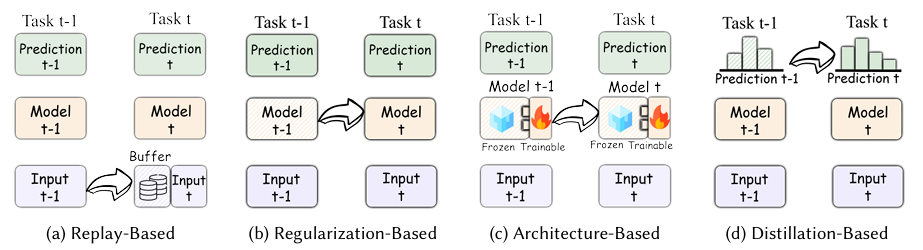
\includegraphics[scale=.45]{Images/Chapter2/llm_methods.png}
\caption[]{طبقه‌بندی روش‌های یادگیری پیوسته در مدل‌های بینایی بزرگ و بینایی-زبان  \protect\cite{llm_continual}}
\label{fig.21}
\end{figure}


\subsection{روش‌های مبتنی بر تنظیم}
در این روش، مدل از مکانیزم‌هایی مانند جریمه یا محدودسازی برای حفظ اطلاعات قبلی استفاده می‌کند. هدف این است که پارامتر‌هایی که در یادگیری گذشته مهم بوده‌اند، هنگام آموزش جدید کمتر تغییر کنند. در این روش، در صورت حجم زیاد وظایف، اثربخشی کاهش می‌یابد
\cite{llm_continual}
.

\subsection{روش‌های مبتنی بر تقطیر دانش}
مدل دانش خود را از مدل‌های قبلی یا معلم یاد می‌گیرد و توجه به مواردی مانند حساسیت به صحت مدل معلم و انتخاب صحیح داده‌ها برای تقطیر حائز اهمیت است
\cite{llm_continual}.
لو و همکاران 
\cite{distillation}،
با هدف کاهش فراموشی در یادگیری افزایشی ویدیو، از روشی به نام تقطیر توجه \LTRfootnote{Attention distillation} استفاده کرده‌اند که در آن ویژگی‌های توجه از خروجی کدگشای ترنسفورمر \lr{CLIP}، به مدل جدید منتقل می‌شود. این رویکرد به مدل کمک می‌کند تا دانش مراحل قبلی را حفظ کرده و در عین حال بتواند دسته‌های جدید را بدون نیاز به آموزش کامل مجدد یاد بگیرد. 


\subsection{روش‌های مبتنی بر معماری}
در این رویکرد، معماری مدل برای جذب وظایف جدید، بدون تداخل با وظایف قبلی، تغییر می‌کند؛ مانند افزودن پیمانه
\LTRfootnote{Module}
 استفاده از تطبیق‌دهنده‌ها و .... 
 ژنگ و همکاران
\cite{llm_continual}،
با بررسی روش‌های مختلف ارائه‌شده در این رویکرد، طبقه‌بندی مطابق با 
\cref{fig.22}
ارائه داده اند که در ادامه به بررسی آن‌ها پرداخته‌ می‌شود
.
\begin{figure}
\centering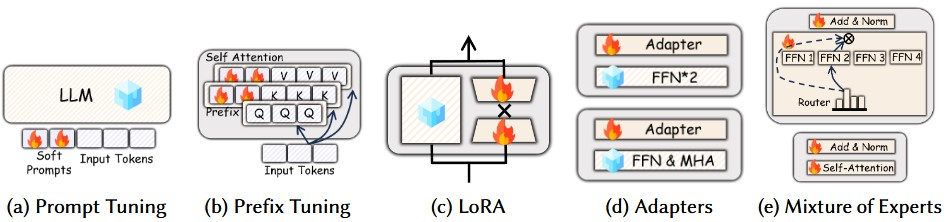
\includegraphics[scale=.75]{Images/Chapter2/llm_architec_methods.jpg}
\caption[]{ روش‌های یادگیری پیوسته مبتنی بر معماری در مدل‌های زبانی بزرگ و بینایی-زبان \protect\cite{llm_continual}}
\label{fig.22}
\end{figure}

\subsubsection{تنظیم پرامپت}
همانطور که در بخش یادگیری انتقالی مدل‌های بینایی-زبان ذکر شد، در روش تنظیم پرامپت، به‌جای بازآموزی کامل یا تغییر در پارامتر‌های اصلی مدل، مجموعه‌ای از بردارهای قابل‌ آموزش به‌عنوان پرامپت به ابتدای نشانه‌های ورودی
\LTRfootnote{Input tokens}
اضافه می‌شوند. این بردارها بدون دست‌کاری در ساختار درونی مدل، نقش راهنما را ایفا کرده و جهت‌گیری مدل در تفسیر داده‌های جدید را مشخص می‌سازند. در واقع، مدل با همان دانش قبلی خود به تحلیل ورودی می‌پردازد، اما به‌واسطه‌ی پرامپت‌های جدید، قادر به تطبیق با وظایف تازه می‌شود \cite{llm_continual}. این روش به‌دلیل مصرف کم منابع محاسباتی و عدم نیاز به تغییر در پارامتر‌های اصلی، به‌ویژه برای سناریوهایی با دسترسی محدود به مدل یا منابع، بسیار مناسب است و الگوی مورد استفاده در این روش، می‌تواند به خوبی برای مسائل یادگیری پیوسته نیز استفاده شود
\cite{llm_continual}.
\begin{figure}
	\centering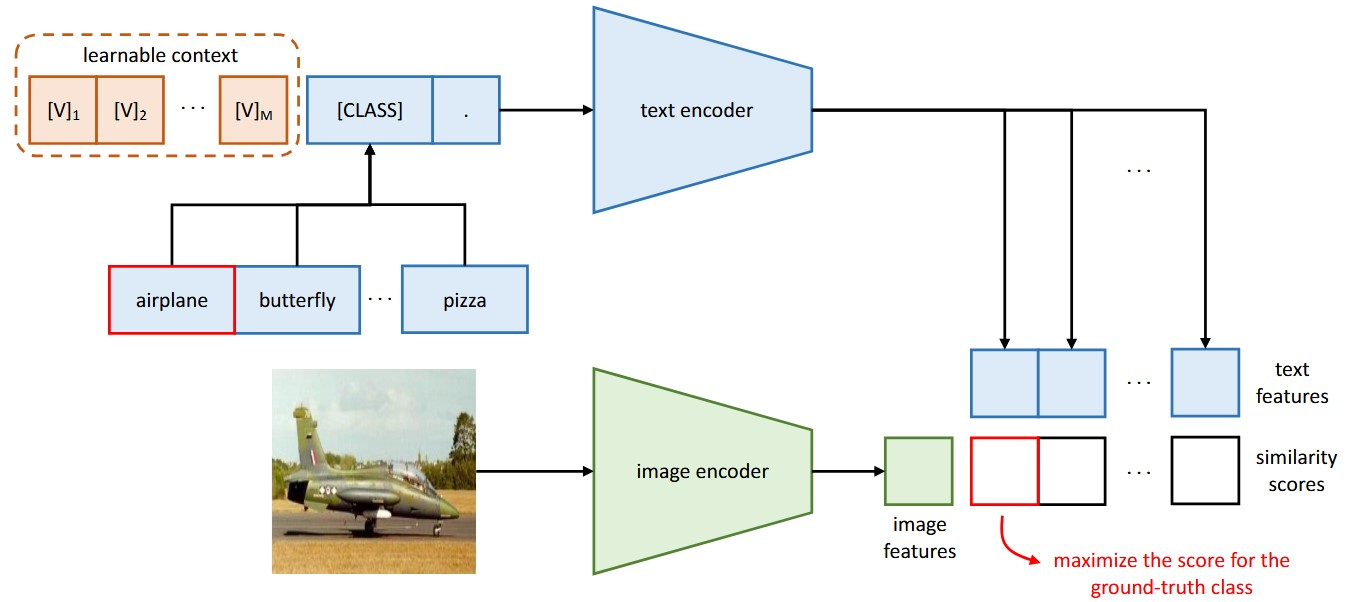
\includegraphics[scale=.55]{Images/Chapter2/CoOp.jpg}
	\caption[]{ نمایش روش 
		\lr{CoOp}
		\protect\cite{CoOp}}
	\label{fig.23}
\end{figure}
\begin{figure}
	\centering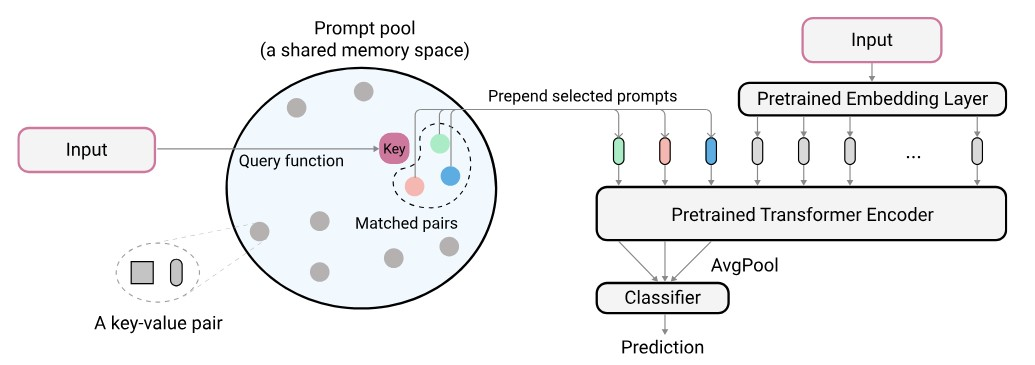
\includegraphics[scale=.65]{Images/Chapter2/l2p.jpg}
	\caption[]{ نمایش روش 
		\lr{L2P}
		در زمان آزمون
		\protect\cite{l2p}}
	\label{fig.24}
\end{figure}
ژو و همکاران 
\cite{CoOp}،
رویکردی به نام بهینه‌سازی بافت 
\LTRfootnote{Context Optimization (CoOp)}
(که در بخش قبل اشاره شد) ارائه کرده‌اند که به جای پرامپت‌های ثابت، از پرامپت به صورت بردارهای بافت یادگرفتنی
\LTRfootnote{Learnable context vectors}
که در کنار برچسب متنی داده‌ها قرار می‌گیرند، استفاده می‌کند. مطابق 
\cref{fig.23}،
تمام وزن‌های مدل 
\lr{CLIP}،
ثابت نگه داشته شده و تنها بردارهای پرامپت، قابل‌آموزش هستند. به دنبال توسعه ی روش های پرامپت گذاری، روش
\lr{L2P}
\LTRfootnote{Learning to Prompt for Continual Learning}
که توسط وانگ و همکاران
\cite{l2p}
ارائه شده است، یک چارچوب نوآورانه برای یادگیری پیوسته بدون نیاز به شناسایی وظیفه در زمان آزمون می‌باشد. همان‌طور که در 
\cref{fig.24}
مشاهده می‌شود، این روش به جای تغییر وزن‌های مدل پیش‌آموخته، از مجموعه‌ای از پرامپت‌های یادگرفتنی بهره می‌برد که در یک فضای حافظه اشتراکی به نام استخر پرامپت
\LTRfootnote{Prompt pool}
نگهداری می‌شوند. 
\lr{L2P}
از یک مکانیزم پرس‌وجوی مبتنی بر جفت‌های کلید-مقدار بهره می‌برد تا به‌صورت پویا و متناسب با ورودی، پرامپت‌های مرتبط را انتخاب کرده و به نشانه‌‌های ورودی مدل، اضافه کند. سپس این نشانه‌‌های توسعه‌یافته به مدل پیش‌آموخته تزریق شده و پیش‌بینی انجام می‌شود.
در این روش، پرامپت‌ها، دانش خاص هر وظیفه یا دانش مشترک بین وظایف را به‌صورت فشرده ذخیره می‌کنند و باعث کاهش چشمگیر فراموشی مخرب در یادگیری وظایف متوالی می‌شوند. ساختار طراحی‌شده در  
\lr{L2P}
همان‌طور که در 
\cref{fig.24}
نشان داده شده، از یک بخش انتخاب پرامپت، لایه‌های کدگذار پیش‌آموخته
\LTRfootnote{Pretrained encoder layers}،
و دسته‌بند نهایی تشکیل شده است. جهت بهبود و مقاوم‌سازی نسبت به فراموشی در انتخاب پرامپت روش‌های پیشین، مارتین و همکاران
\cite{starprompt}،
روش 
\lr{STAR-Prompt}
را معرفی کرده‌اند که از رویکردی دوسطحی برای تنظیم پرامپت، پیروی می‌کند. ابتدا از 
\lr{CLIP}،
برای تولید پرامپت‌های متنی و ساخت نمونه‌های‌ اولیه
\LTRfootnote{Prototypes}
پایدار دسته‌ها، استفاده می‌شود و سپس این نمونه‌های اولیه به‌عنوان کلید برای بازیابی پرامپت‌های تصویری در ترنسفورمر تصویر به‌کار می‌روند. هم‌چنین روش‌های
\lr{DualPrompt}
\cite{dual-prompt}
و 
\lr{H-prompts}
\cite{h-prompts}،
مانند مطالعات مذکور، در زمینه‌ی تولید پرامپت‌های مشترک و خاص وظایف ارائه شده‌اند. داهویین و همکاران
\cite{instance_prompt}،
از پرامپت اختصاصی برای هر نمونه به‌جای هر‌دسته، استفاده کرده‌اند. برخلاف روش‌های پرامپت‌گذاری قبلی، هنگ و همکاران
\cite{ovor}،
علاوه بر استفاده از یک پرامپت به‌جای چندپرامپت، از نمونه‌های پرت مصنوعی برای ایجاد مرز دسته‌بندی بهتر استفاده کرده‌اند. در مطالعات دیگری مانند روش یکپارچه‌سازی دانش بدون تداخل و آگاه از توزیع
\cite{diki}
\LTRfootnote{Distribution-aware Interference-free Knowledge Integration (DIKI)}،
به رفع چالش مداخله‌ی پرامپت در تصمیم‌گیری مکانیزم توجه پرداخته شده است. به دنبال پیشرفت‌های روش‌های پرامپت در حوزه‌ی تصویر، ویلا و همکاران
\cite{pivot}،
روشی به نام
\lr{PIVOT}
را معرفی کرده‌اند که با بهره‌گیری از دانش پیش‌آموخته مدل‌ تصویر-متن
\lr{CLIP}
و استفاده از پرامپت‌های مکانی
\LTRfootnote{Spatial prompts}
و زمانی، وابستگی‌های زمانی و مکانی ویدیوها را مدل کرده است. وانگ و همکاران \cite{clip-poolprompt} نیز با هدف ارتقای عملکرد مدل \lr{CLIP} در تشخیص حرکت‌های انسانی در ویدیوها، چارچوبی معرفی کرده‌اند که با استفاده از مدل‌سازی حرکتی و پرامپت‌های پویا، به شکلی مؤثر اطلاعات حرکتی را وارد فرآیند یادگیری می‌کند بدون اینکه به تغییر پارامتر‌های اصلی \lr{CLIP} نیاز باشد. در مواردی نیز مانند روش \lr{ViLT-CLIP} 
\cite{vilt-clip}،
از هر دو نوع پرامپت برای تصویر و متن برای درک ویژگی‌های ویدیویی استفاده شده‌است.

 
\subsubsection{تنظیم پیشوند}
 در روش تنظیم پیشوند \LTRfootnote{Prefix tuning}، مجموعه‌ای از پارامتر‌های قابل آموزش به عنوان پیشوند به ابتدای هر لایه‌ی ترنسفورمر افزوده می‌شود تا رفتار مدل را در انجام وظایف خاص تنظیم کند. این پیشوندها نقش تغییرات زمینه‌ای را ایفا کرده و برخلاف تنظیم پرامپت، چندین لایه از مدل را تحت تأثیر قرار می‌دهند \cite{llm_continual}. روی و همکاران \cite{prefix-tuning}، روشی معرفی کرده‌اند که با استفاده از پیشوندهای قابل یادگیری در هر لایه‌ی مدل، امکان یادگیری وظایف جدید را بدون فراموشی وظایف قبلی فراهم می‌کند. این پیشوندها با ترکیب کانولوشن و اطلاعات مشترک بین وظایف، باعث انتقال بهتر دانش و کاهش تعداد پارامتر‌های لازم در یادگیری پیوسته می‌شوند.
 
\subsubsection{سازگار‌سازی رتبه‌پایین}
 با وارد کردن ماتریس‌های رتبه‌پایین در لایه‌های معینی از مدل پیش‌آموخته و منجمد، روش سازگار‌سازی رتبه‌پایین \LTRfootnote{Low‑Rank Adaptation (LoRA)}، امکان تنظیم هدفمند بخش‌هایی از مدل را بدون بازآموزی کامل فراهم می‌سازد \cite{llm_continual}. مارتین و همکاران \cite{lora}، به نتیجه رسیدند که در زمینه‌ی یادگیری پیوسته، جایگزینی روش مذکور به‌جای تنظیم پرامپت، بدون افزایش چشمگیر در تعداد پارامتر‌ها، منجر به بهبود عملکرد مدل می‌گردد.
 
\subsubsection{وفق دهنده}
همانطور که در بخش یادگیری انتقالی مدل‌های بینایی-زبان ذکر شد، وفق دهنده‌ها شبکه‌های عصبی کوچک با ساختار فشرده‌ای هستند که بین لایه‌های مدل اصلی قرار می‌گیرند و به مدل امکان می‌دهند ویژگی‌های جدید را یاد بگیرد، بدون آن‌که نیازی به تغییر پارامتر‌های اصلیِ از پیش آموزش‌دیده باشد \cite{llm_continual}. به همین دلیل، می‌توان این روش را نیز در یادگیری پیوسته استفاده نمود. در برخی روش‌ها مانند 
\lr{DIA}
\cite{dia-adapter-2025}
و 
\lr{EASE}
\cite{ease-adapter-2024}،
از وفق دهنده‌های سبک‌وزن و اختصاصی برای هر وظیفه‌ی جدید استفاده می‌شود تا مدل بتواند بدون بازآموزی کامل یا ذخیره داده‌های قدیمی، دانش جدید را جذب کند. این دو روش، امکان به‌روزرسانی مدل را بدون آسیب به دانش قبلی فراهم کرده و تصمیم‌گیری ترکیبی میان دسته‌های قدیم و جدید را ممکن می‌سازند. دانگ و همکاران 
\cite{cada-adapter-2025}،
در مطالعه‌ای دیگر، روشی به نام \lr{C-ADA}، ارائه داده‌اند که با استفاده از وفق دهنده‌هایی با قابلیت گسترش عاملی، یادگیری وظایف جدید را بدون نیاز به ذخیره داده‌های گذشته ممکن می‌سازد. این روش با حفظ پارامتر‌های قبلی و افزودن وزن‌های جدید، از تداخل دانش جلوگیری کرده و عملکرد و سرعت آموزش را به‌طور محسوسی بهبود می‌دهد. برای رفع چالش تداخل پارامتر‌های دسته‌های مشابه در یادگیری پیوسته، هانگ و همکاران 
\cite{rapf-adapter-2024}،
با استفاده از وفق دهنده‌های قابل تنظیم، ابتدا بازنمایی‌های متنی را متناسب با تأثیر دسته‌های جدید بر دسته‌های قدیمی اصلاح می‌کنند و سپس با یک راه‌برد تجزیه و ادغام پارامتر‌ها، فراموشی مدل در حین تنظیم وفق دهنده‌ها را کاهش می‌دهند. در حوزه‌ی ویدیو نیز، پن و همکاران 
\cite{st-adapter-2022}،
روشی به نام \lr{ST-Adapter} پیشنهاد داده‌اند که با افزودن قابلیت زمانی-مکانی به مدل‌ تصویری از پیش‌آموخته، آن را برای وظایف ویدیویی قابل استفاده کرده است. 
 
\subsubsection{مخلوط خبره‌ها}
 روش مخلوط خبره‌ها
\LTRfootnote{Mixture of Experts (MoE)}،
 با استفاده از یک مکانیزم دروازه‌ای، به‌صورت پویا تعدادی از شبکه‌های عصبی خبره را برای انجام هر وظیفه فعال می‌کند. این ساختار باعث می‌شود مدل بخش‌های مختلف خود را به وظایف متنوع اختصاص دهد و عملکرد بهتر و مقیاس‌پذیری بیشتری پیدا کند. ونگ و همکاران 
\cite{sema-2024}،
در این زمینه رویکردی را ارائه داده‌اند که مدل به‌صورت خودکار تصمیم می‌گیرد که بسته به تغییر داده یا وظیفه، از کدام وفق دهنده‌های موجود استفاده کند یا وفق دهنده‌ی جدیدی اضافه نماید، تا تعادلی میان حفظ دانش قبلی و یادگیری دانش جدید ایجاد شود. در ادامه نیز، یو و همکاران 
\cite{ddas-2024}،
با استفاده از همین روش و با گسترش تدریجی مدل \lr{CLIP} و استفاده از مسیرهای انتخابی میان وفق دهنده‌های خبره و مدل اصلی، قابلیت تشخیص یادگیری بدون نمونه حفظ شده و در عین حال بار محاسباتی به شکل چشم‌گیری کاهش می‌یابد.

 
\section{جمع‌بندی}
در این فصل، به بررسی یادگیری پیوسته با تمرکز بر حوزه‌های تصویر، ویدیو و مدل‌های بینایی-زبان پرداخته شد. ابتدا مفهوم یادگیری پیوسته معرفی شد که هدف آن توانایی سیستم‌های هوشمند در کسب و به‌روزرسانی دانش در طول زمان بدون فراموش کردن دانش پیشین است. این حوزه با چالش اصلی «فراموشی فاجعه‌بار» روبه‌روست؛ مشکلی که هنگام ورود داده‌های جدید، باعث تضعیف یا حذف دانش قبلی مدل می‌شود.

رویکردهای اصلی مقابله با این چالش در چهار دسته‌ی مبتنی بر تنظیم، بازپخش، بهینه‌سازی و معماری طبقه‌بندی شدند. هر یک از این روش‌ها مزایا و محدودیت‌های خاص خود را دارند، از جمله استفاده از حافظه خارجی برای بازپخش داده‌های قدیمی، یا تنظیم پارامتر‌ها برای حفظ دانش پیشین.

همچنین، مدل‌های بینایی-زبان معرفی و بررسی شدند. این مدل‌ها با ترکیب اطلاعات تصویری و متنی، قادر به درک عمیق‌تری از محتوای چندرسانه‌ای هستند و در وظایفی مانند توصیف تصاویر، پرسش‌وپاسخ تصویری و جستجوی مبتنی بر تصویر نقش مهمی ایفا می‌کنند. ادغام این مدل‌ها با رویکردهای یادگیری پیوسته، نیازمند راهکارهایی برای مدیریت همزمان دانش در هر دو حوزه بینایی و زبان است.

در مجموع، این فصل اهمیت یادگیری پیوسته در توسعه سامانه‌های هوشمند را برجسته کرد و نشان داد که طراحی روش‌های نوآورانه برای مدیریت داده‌های جدید و حفظ اطلاعات پیشین، به‌ویژه در مدل‌های بینایی-زبان، یکی از محورهای کلیدی پیشرفت در هوش مصنوعی آینده است.
 
 
 
 
 
 
 
 
 
 
 
 
 
 
 
 
 
 
 
 
 
 
 
 
